\documentclass[t]{beamer}
\usepackage{lmodern} % Need to use this package for proper font encoding.
\usepackage[T1]{fontenc}
\usepackage{amsmath}
\usepackage{graphicx}

% Title slide information
\title{Evaluation of Gene Finding Tools on \textit{Trichoderma} Genomes - Update}
\date{July, 2025} 
\author{Connor Burbridge}
\titlegraphic{UsaskAerial.jpg} 
\institute{Department of Computer Science} 
\usetheme{usask}

\begin{document}

\begin{frame}
	\titlepage
\end{frame}

%%%%%%%%%%%%%%%%%
\begin{frame}
	\frametitle{Outline} 

	\begin{itemize}
		\item Progress update with results
		\item Progress assessment
		\item Timeline for completion	
		\item Discussion of next steps
	\end{itemize}
\end{frame}

%%%%%%%%%%%%%%%%
\begin{frame}
	\frametitle{Background} 
	\begin{itemize}
		\item Gene finding is a critical step in genome annotation.
		\item \textit{Trichoderma} species are important for agriculture and biotechnology.
		\item Various tools exist for gene prediction, but their implementations and performance can vary significantly.
		\item Few studies have compared these tools in fungi, and even fewer in \textit{Trichoderma}.
		\item In addition, high-quality reference genomes are not available for all species, which makes comparisons difficult.
	\end{itemize}
\end{frame}

\begin{frame}
	\frametitle{Why \textit{Trichoderma}?}
	\begin{itemize}
		\item \textit{Trichoderma} species are ubiquitous in soil and play a significant role in nutrient cycling.
		\item They are also used in biocontrol and as biofertilizers.
		\item Known for their production of plant cell wall degrading enzymes, and secondary metabolites.
		\item Further genomic studies can help in understanding their biology and potential applications.
	\end{itemize}
\end{frame}

\begin{frame}
	\frametitle{Novel \textit{Trichoderma} Genomes}
	\begin{itemize}
		\item \textit{Trichoderma} species are diverse, with many species not yet fully characterized.
		\item Recent advances in sequencing technology have made it possible to generate high-quality genomes for these species.
		\item Two novel genomes of \textit{Trichoderma} species have been sequenced at the Global Institute for food Security
		\item DC1 and Tsth20, shown to improve drought and salt tolerance when applied to crops.
		\item These genomes provide an opportunity to evaluate gene finding tools in a comparative context, and contribute to the understanding of \textit{Trichoderma} biology. 
	\end{itemize}
\end{frame}

\begin{frame}
	\frametitle{Workflow Overview}
	\centering
	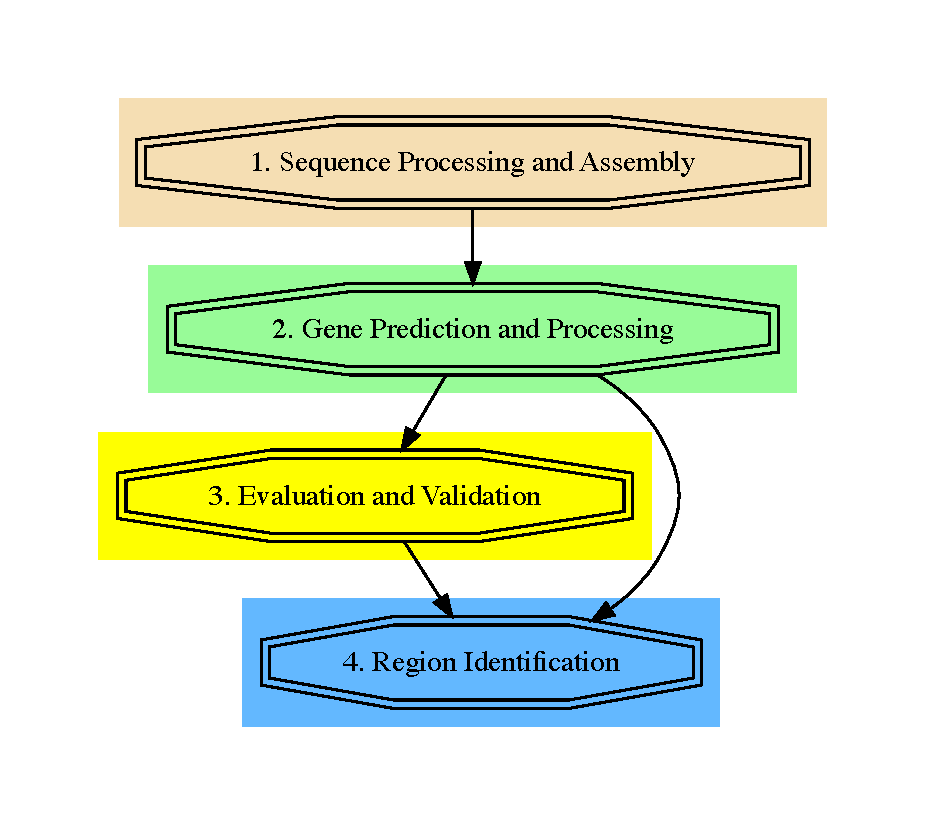
\includegraphics[width=0.9\textwidth]{../../working-thesis/figures/workflow-simple.pdf}
\end{frame}

\begin{frame}
	\frametitle{Datasets and Tools}
	\begin{itemize}
		\item \textbf{Datasets:}
		\begin{itemize}
			\item \textit{Trichoderma} genomes: DC1 and Tsth20.
			\item Reference genomes and annotations: \textit{T. reesei, T. harzianum, T.virens}.
			\item RNAseq training data from \textit{T. reesei}. 
			\item Benchmarking Universal Single-Copy Orthologs (BUSCO) fungal database.
			\item Protein sequence queries for tblastn from \textit{T. atroviride, Fusarium graminearum, and Saccharomyces cerevisiae}.	
		\end{itemize}
		\item \textbf{Tools:}
		\begin{itemize}
			\item Sequence processing: FastQC, Trimmomatic, Hisat2.
			\item Genome assembly: NextDenovo and NextPolish.
			\item Gene finding tools: Braker2 and GeneMark-ES.
			\item Evaluation tools: BUSCO, tblastn, InterProScan, and custom scripts.
		\end{itemize}
	\end{itemize}
\end{frame}

\begin{frame}
	\frametitle{Assembly Results}
	\centering
	\vspace{0.5cm}
	\resizebox{\linewidth}{!}{
    \begin{tabular}{|c|c|c|c|c|c|c|}
		\hline
  		Name & Total Contigs & Total Length & Largest Contig & GC\% & N50 & L50 \\ \hline
     	DC1 & 8 & 38.6 Mb & 11.49 Mb & 47.97 & 5.69 Mb & 3 \\ \hline
      	Tsth20 & 7 & 41.58 Mb & 8.02 Mb & 47.33 & 6.52 Mb & 3 \\ \hline
      	\textit{T. harzianum} & 532 & 40.98 Mb & 4.08 Mb & 47.61 & 2.41 Mb & 7 \\ \hline
      	\textit{T. virens} & 93 & 39.02 Mb & 3.45 Mb & 49.25 & 1.83 Mb & 8 \\ \hline
      	\textit{T. reesei} & 77 & 33.39 Mb & 3.75 Mb & 52.82 & 1.21 Mb & 9 \\ \hline
    \end{tabular}}
	\begin{itemize}
		\item DC1 and Tsth20 assemblies are high quality with few contigs in comparison to other \textit{Trichoderma} assemblies.
		\item Input sequences and assemblies show a bimodal distribution of GC content.
		\item AT-rich sequence content may be related to transposable elements and repeat-induced mutations, which may be of interest in secondary metabolite production.
	\end{itemize}
\end{frame}

\begin{frame}
	\frametitle{Gene Finding Results}
	\centering
	\resizebox{\linewidth}{!}{
	\begin{tabular}{|c|c|c|c|c|c|c|}
    	\hline
    	Assembly & Braker2 & & GeneMark & & RefSeq & \\ \hline
     	& Genes & CDS & Genes & CDS & Genes & CDS \\ \hline
    	DC1 & 8546 & 8637 & 11353 & 11353 & N/A & N/A \\ \hline
    	Tsth20 & 8784 & 8858 & 12362 & 12362 & N/A & N/A \\ \hline
    	\textit{T. reesei} & 9659 & 10175 & 9196 & 9196 & 9109 & 9118 \\ \hline
    	\textit{T. harzianum} & 8314 & 8385 & 12164 & 12164 & 14269 & 14090 \\ \hline
    	\textit{T. virens} & 7801 & 7863 & 11866 & 11866 & 12405 & 12406 \\ \hline
  	\end{tabular}}
	\begin{itemize}
		\item Braker2 predicts more genes and coding sequences than GeneMark and RefSeq in \textit{T. ressei}, but fewer in other assemblies.
		\item GeneMark and RefSeq predictions are similar, except in \textit{T. harzianum}, where RefSeq predicts 17\% more genes.
		\item GeneMark only predicts one coding sequence per gene, while Braker2 and RefSeq predict multiple coding sequences.
	\end{itemize}
\end{frame}

\begin{frame}
	\frametitle{Examining Coding Sequence Lengths}
	\centering
	\vspace{0.3cm}
	\resizebox{0.9\linewidth}{!}{
	\begin{tabular}{|c|c|c|c|c|c|c|}
      \hline
      Genome & Tool \#1 & Tool \#2 & \textit{P}-value  \\ \hline
      DC1 & Braker2 & GeneMark & $0.999$ \\ \hline
      Tsth20 & Braker2 & GeneMark & $0.965$ \\ \hline
      \textit{T. reesei} & Braker2 & GeneMark & $9.481*10^{-07}$ \\ \hline
      \textit{T. reesei} & GeneMark & RefSeq & $0.002$ \\ \hline
      \textit{T. reesei} & Braker2 & RefSeq & $1.340*10^{-07}$ \\ \hline
      \textit{T. harzianum} & Braker2 & GeneMark & $0.863$ \\ \hline
      \textit{T. harzianum} & GeneMark & RefSeq & $4.313*10^{-52}$ \\ \hline
      \textit{T. harzianum} & Braker2 & RefSeq & $4.674*10^{-55}$ \\ \hline
      \textit{T. virens} & Braker2 & GeneMark & $0.635$ \\ \hline
      \textit{T. virens} & GeneMark & RefSeq & $7.352*10^{-12}$ \\ \hline
      \textit{T. virens} & Braker2 & RefSeq & $1.794*10^{-09}$ \\ \hline
    \end{tabular}}
\end{frame}


\begin{frame}
	\frametitle{BUSCO Results}
	\centering
	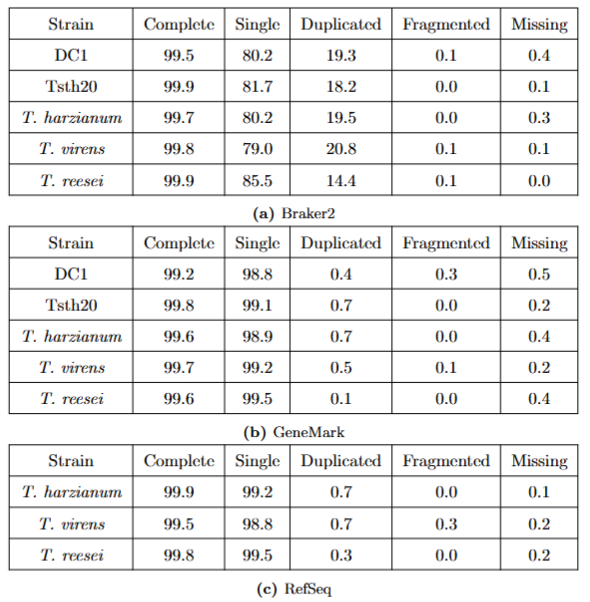
\includegraphics[width=0.65\textwidth]{../../working-thesis/figures/busco-screenshot.png}
\end{frame}

\begin{frame}
	\frametitle{Agreement of Gene Predictions}
	\centering
	\begin{itemize}
		\item In DC1 and Tsth20, BRaker2 and GeneMark tend to agree on theh start and stop positions of genes when they predict the same gene. Both gene finders have a large portion of singleton predictions.
	\end{itemize}
	\begin{figure}
		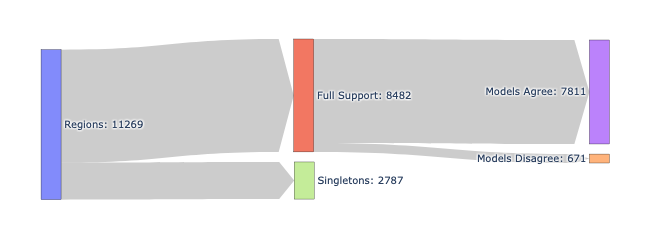
\includegraphics[width=0.9\textwidth]{../../working-thesis/figures/dc1-region-breakdown.png}
		\caption{DC1}
	\end{figure}
\end{frame}

\begin{frame}
	\vspace{1cm}
	\centering
	\begin{itemize}
		\item In \textit{T. reesei}, Braker2, GeneMark and RefSeq tend to disagree more on the start and stop positions of genes when they predict the same gene.
		\item Disagreement is more pronounced in \textit{T. harzianum} and \textit{T. virens}, where genes with partial support from more than one gene finder are common.
		
	\end{itemize}
	\begin{figure}
		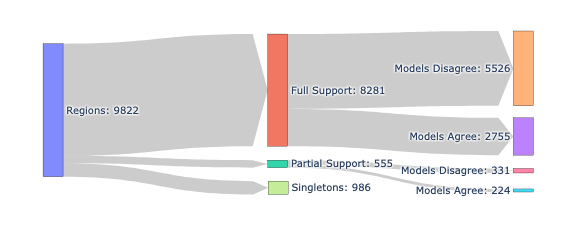
\includegraphics[width=0.8\textwidth]{../../working-thesis/figures/t-reesei-region-breakdown.png}
		\caption{\textit{T. reesei}}
	\end{figure}
\end{frame}

\begin{frame}
	\frametitle{InterProScan Results}
	\centering
	\begin{itemize}
		\item k
	\end{itemize}
	\resizebox{\linewidth}{!}{
	\begin{tabular}{|c|c|c|c|c|c|c|}
    \hline
    Assembly & Braker2 & GeneMark & RefSeq \\ \hline
DC1 & $\frac{10676}{14479}$ & $\frac{8416}{11354}$ & \
N/A \\ \hline
    Tsth20 & $\frac{11389}{15546}$ & $\frac{9168}{12373}$\
 & N/A \\ \hline
    \textit{T. reesei} & $\frac{8471}{11704}$ & $\frac{6990}{9196}$ & $\frac{6964}{9111}$ \\ \hline
    \textit{T. harzianum} & $\frac{11370}{15408}$ & $\frac{9061}{12164}$ & $\frac{9293}{14065}$ \\ \hline
    \textit{T. virens} & $\frac{11249}{15062}$ & $\frac{8871}{11866}$ & $\frac{9062}{12383}$ \\ \hline
  \end{tabular}}
\end{frame}

\end{document}